\documentclass{../../slides-style}

\slidetitleext{Лекция 8: Работа в команде}{11.04.2023}{Работа в команде}

\begin{document}

    \begin{frame}[plain]
        \titlepage
    \end{frame}

    \section{Команда}

    \begin{frame}
        \frametitle{Что такое команда?}
        \begin{itemize}
            \item Люди должны кооперироваться, чтобы выполнять свои задачи
            \item Продукт или сервис в целом не равен сумме отдельных его частей
        \end{itemize}
    \end{frame}

    \begin{frame}
        \frametitle{Высокоэффективная команда --- это сложно!}
        \begin{itemize}
            \item Разный уровень работы сообща
            \item Разный профессиональный уровень
            \item Разный уровень культуры
            \item Разные темпераменты
            \item Разные подходы к решению задач
            \item Личные отношения
            \item ...
        \end{itemize}
    \end{frame}

    \begin{frame}
        \frametitle{Составляющие успешной команды}
        \begin{center}
            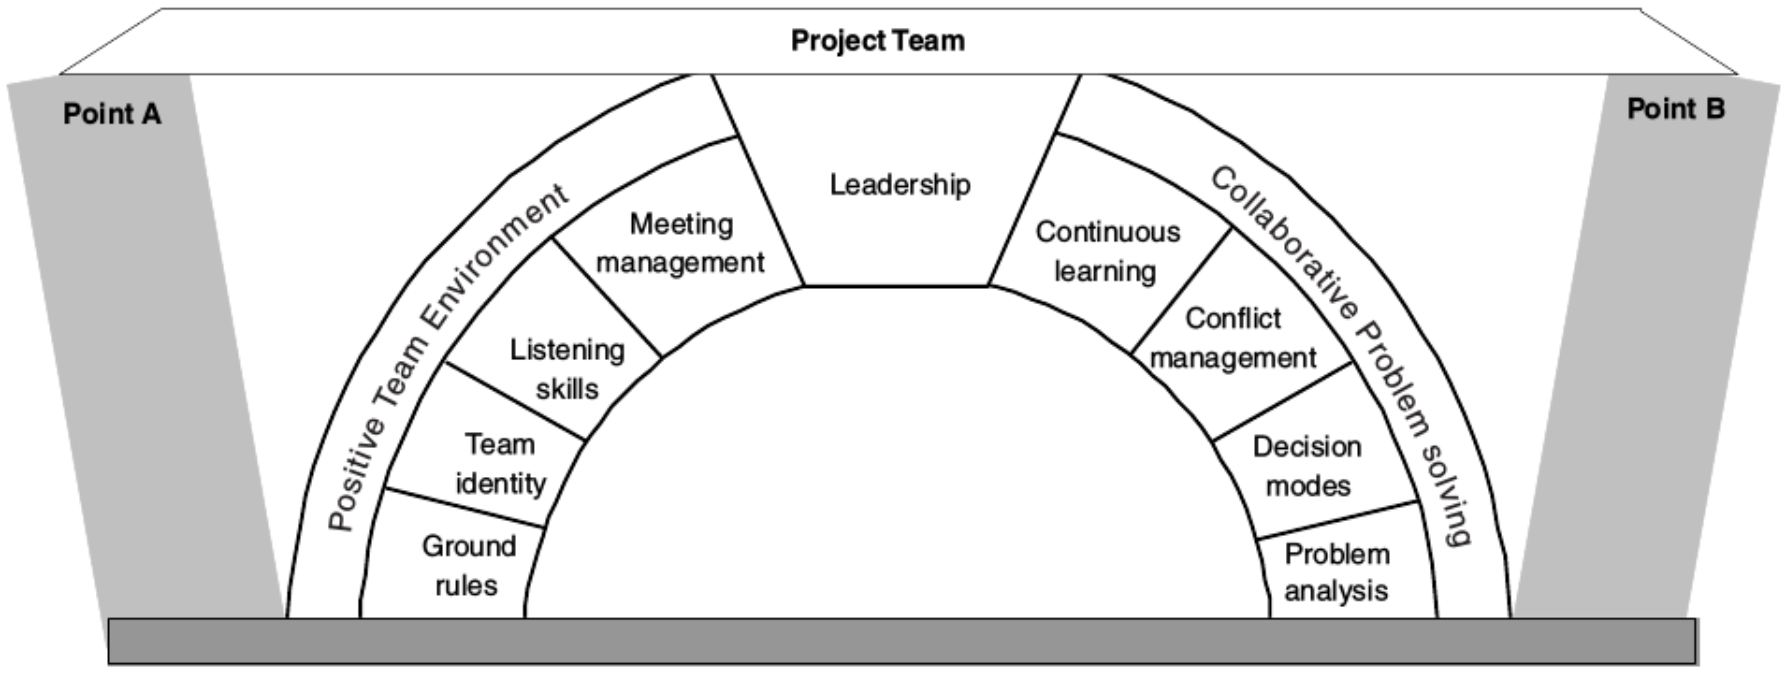
\includegraphics[width=0.95\textwidth]{successfulTeamComponents.png}
        \end{center}
    \end{frame}

    \section{Позитивная экосистема}

    \begin{frame}
        \frametitle{Позитивная экосистема команды}
        \begin{itemize}
            \item Набор базовых правил 
            \item Сплочённость команды
            \item Умение слушать
            \item Умение проводить совещания
        \end{itemize}
    \end{frame}

    \begin{frame}
        \frametitle{Базовые правила}
        \begin{itemize}
            \item Позволяют структуризовать команду
            \item Определяют внутреннюю культуру
            \item Формируют ожидания членов команды
        \end{itemize}
    \end{frame}

    \begin{frame}
        \frametitle{Пример списка правил}
        \begin{itemize}
            \item Соблюдение конфиденциальности
            \item Поощрение обучения
            \item Взаимоуважение
            \item Дисциплина обязательств
            \item Проведение совещаний
            \begin{itemize}
                \item Активное слушание
                \item Ориентация на результат
                \item Пунктуальность
                \item Минимум отвлечений
                \item Подготовленность
            \end{itemize}
        \end{itemize}
    \end{frame}

    \begin{frame}
        \frametitle{Сплочённость команды}
        \begin{itemize}
            \item Понимание целей проекта членами команды
            \begin{itemize}
                \item Понимание потребностей заказчика/пользователей
            \end{itemize}
            \item Ощущение поддержки со стороны руководства
            \item Понимание сильных сторон и особенностей друг друга
            \item И не стоит забывать:
            \begin{itemize}
                \item Собеседования
                \item Регулярные встречи “вживую”
                \item Тимбилдинг
                \item Печеньки!
            \end{itemize}
        \end{itemize}
    \end{frame}

    \begin{frame}
        \frametitle{Умение слушать}
        \begin{itemize}
            \item Активное слушание
            \begin{itemize}
                \item Отсутствие отвлекающих факторов
                \item Непредвзятость
                \item Стиль подачи материала
                \item Фокусировка на процессе
            \end{itemize}
            \item Отсутствие преждевременных суждений
        \end{itemize}
    \end{frame}

    \begin{frame}
        \frametitle{Умение проводить совещания}
        \begin{itemize}
            \item До
            \begin{itemize}
                \item Приглашение
                \item Повестка
            \end{itemize}
            \item Во время
            \begin{itemize}
                \item Пунктуальность
                \item Следование повестке
                \item Наличие секретаря
                \item Участие всех заинтересованных
            \end{itemize}
            \item В конце
            \begin{itemize}
                \item Резюме
                \item Пунктуальность!!!
            \end{itemize}
            \item После
            \begin{itemize}
                \item Протокол (minutes)
            \end{itemize}
        \end{itemize}
    \end{frame}

    \section{Совместное решение задач}

    \begin{frame}
        \frametitle{Совместное решение задач}
        \begin{itemize}
            \item Анализ задач
            \item Варианты принятия решений
            \item Разрешение конфликтов
            \item Непрерывное обучение
        \end{itemize}
    \end{frame}

    \begin{frame}
        \frametitle{Анализ задач}
        \begin{center}
            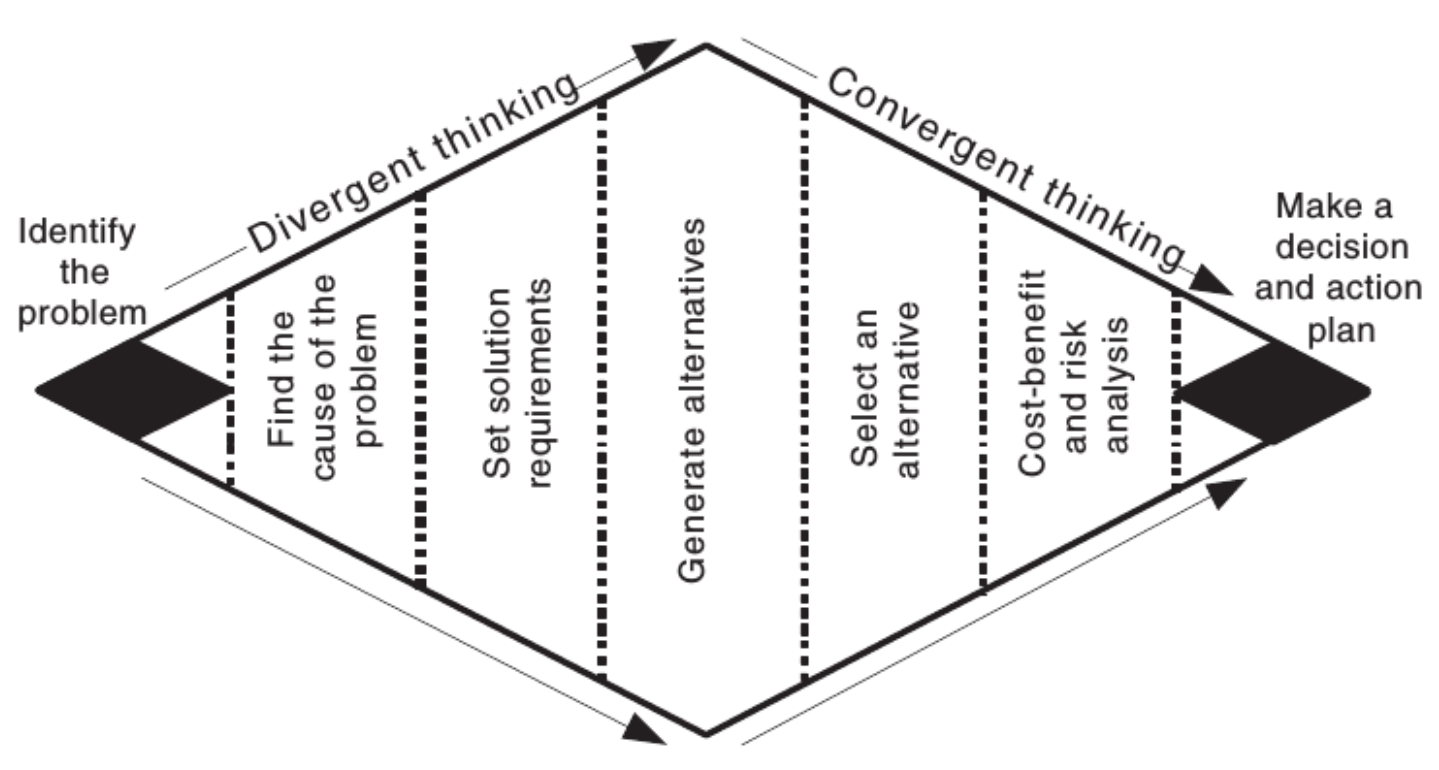
\includegraphics[width=0.8\textwidth]{taskAnalysis.png}
        \end{center}
    \end{frame}

    \begin{frame}
        \frametitle{Варианты принятия решений}
        \begin{itemize}
            \item Консенсус
            \item Голосование
            \item Делегирование
            \item Автократия
        \end{itemize}
    \end{frame}

    \section{Разрешение конфликтов}

    \begin{frame}
        \frametitle{Разрешение конфликтов}
        \begin{itemize}
            \item Конфликты --- это нормально!
            \begin{itemize}
                \item Если без фанатизма
            \end{itemize}
            \item Варианты решения
            \begin{itemize}
                \item Предотвращение
                \item Уход от конфликта
                \item Сглаживание конфликта
                \item Насаждение силой
                \item Компромисс
                \item Конфронтация конфликта
                \begin{itemize}
                    \item Признание конфликта
                    \item Определение контекста и целей
                    \item Определение и выбор альтернатив
                    \item План Б
                \end{itemize}
            \end{itemize}
        \end{itemize}
    \end{frame}

    \section{Непрерывное обучение}

    \begin{frame}
        \frametitle{Непрерывное обучение}
        \begin{itemize}
            \item Улучшение культуры команды
            \item Вовлечение членов команды в процессы проекта
            \item Открытость и честность
            \item Регулярная переоценка и обратная связь
            \item Технический рост
            \item Пересмотр целей и планов проекта
        \end{itemize}
    \end{frame}

    \section{Формирование команды}

    \begin{frame}
        \frametitle{Особенности формирования команды}
        \begin{itemize}
            \item Подбор подходящих людей
            \begin{itemize}
                \item Суперзвёзды, простые смертные, новички
                \item Различные темпераменты
                \item Различные роли в команде
                \item Личные характеристики
                \item Регулировка численности команды
                \item Различные специальности и компетенции
                \begin{itemize}
                    \item Не забыть про QA
                \end{itemize}
            \end{itemize}
            \item Подходящее помещение
            \begin{itemize}
                \item Кабинеты, кубики, опенспейс
            \end{itemize}
            \item Поддержание командного духа
        \end{itemize}
    \end{frame}

    \begin{frame}
        \frametitle{Важные личные характеристики}
        \begin{itemize}
            \item Внутренняя/внешняя управляемость
            \item Высокая/низкая мотивация
            \item Умение быть точным
            \item Исполнительность
            \item Терпимость к неопределенности
            \item Эгоизм
            \item Степень увлеченности
            \item Склонность к риску
            \item Самооценка
            \item Личные отношения в коллективе
        \end{itemize}
    \end{frame}

    \section{Командная разработка}

    \begin{frame}
        \frametitle{Командная разработка ПО}
        \begin{columns}
            \begin{column}{0.6\textwidth}
                \begin{itemize}
                    \item Стиль оформления
                    \item Тесты
                    \item Документирование
                    \item Версии библиотек и инструментов
                    \begin{itemize}
                        \item Третьесторонние библиотеки
                    \end{itemize}
                    \item Ревью
                    \begin{itemize}
                        \item Design review
                        \item code review
                    \end{itemize}
                \end{itemize}
            \end{column}
            \begin{column}{0.4\textwidth}
                \begin{center}
                    
\includegraphics[height=0.8\textheight]{documentation.png}
                \end{center}
            \end{column}
        \end{columns}
    \end{frame}

    \begin{frame}
        \frametitle{Ревью кода}
        \begin{itemize}
            \item Цель --- сделать код лучше
            \begin{itemize}
                \item Но не в ущерб проекту
            \end{itemize}
            \item Просмотры кода
            \item Pre- и post-commit review
            \item Раунды инспекций
            \item Доносим изменение кода правильно
            \begin{itemize}
                \item Работоспособность, размер, стиль, описание
            \end{itemize}
            \item Доносим своё мнение правильно
            \begin{itemize}
                \item Скорость, благожелательность, 
                \item Декларативность, приоритеты замечаний
            \end{itemize}
            \item Мир костылей vs Перфекционизм
        \end{itemize}
    \end{frame}

    \section{Системы контроля версий}

    \begin{frame}
        \frametitle{Работа с системой контроля версий}
        \begin{center}
            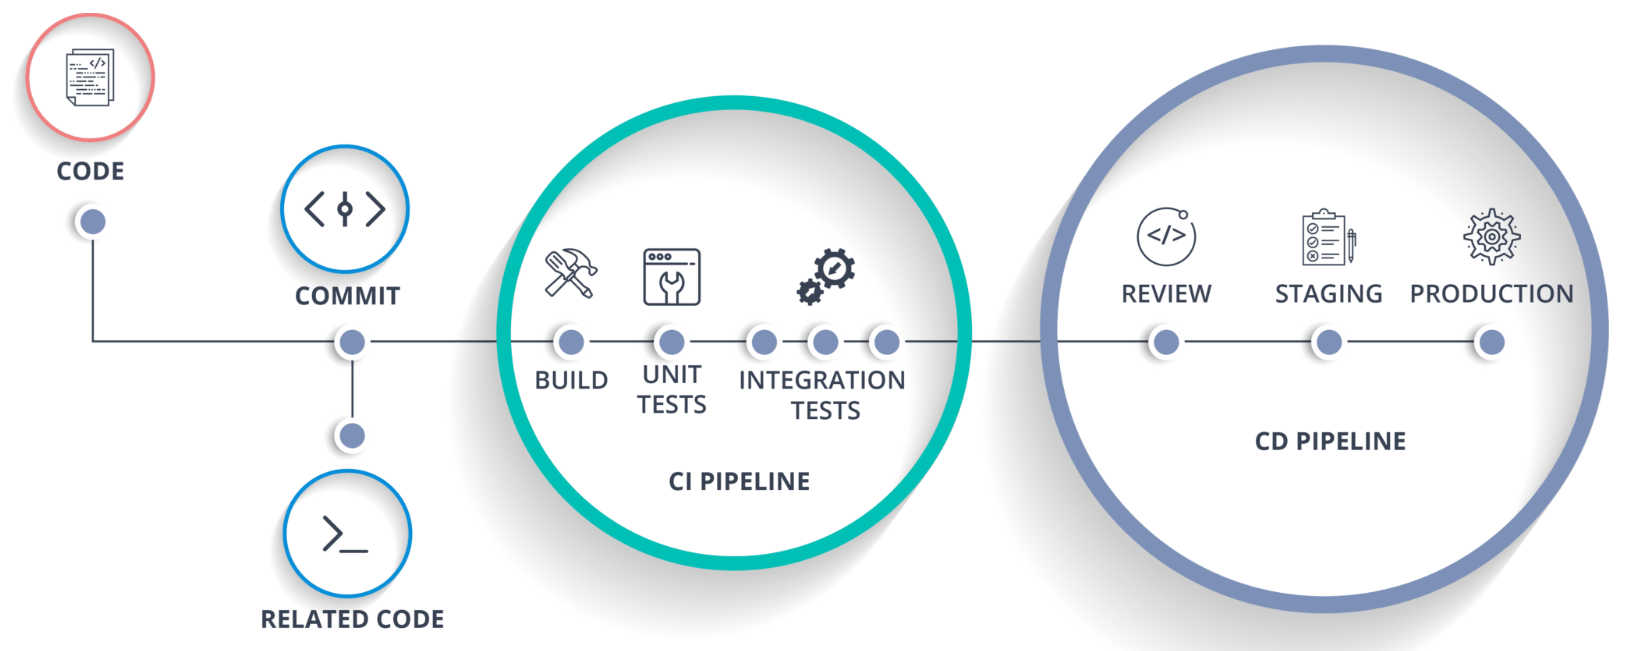
\includegraphics[width=0.8\textwidth]{vcsPipeline.png}
        \end{center}
    \end{frame}

    \begin{frame}
        \frametitle{Модели ветвления}
        \begin{itemize}
            \item Разработка в главной ветке
            \item Gitflow
            \item GitHub flow
            \item GitLab flow
            \item OneFlow
        \end{itemize}
    \end{frame}

    \begin{frame}
        \frametitle{Разработка в главной ветке}
        \begin{itemize}
            \item Избежание ``merging hell''
            \item Инкрементальная разработка
            \item Частые коммиты (хотя бы раз в день)
            \begin{itemize}
                \item Не каждый коммит может попасть в релиз
            \end{itemize}
            \item Сокрытие неготовой функциональности
            \item Допускаются релизные или другие самостоятельные ветки
        \end{itemize}
    \end{frame}

    \subsection{Gitflow}

    \begin{frame}
        \frametitle{Gitflow, main и develop}
        \begin{center}
            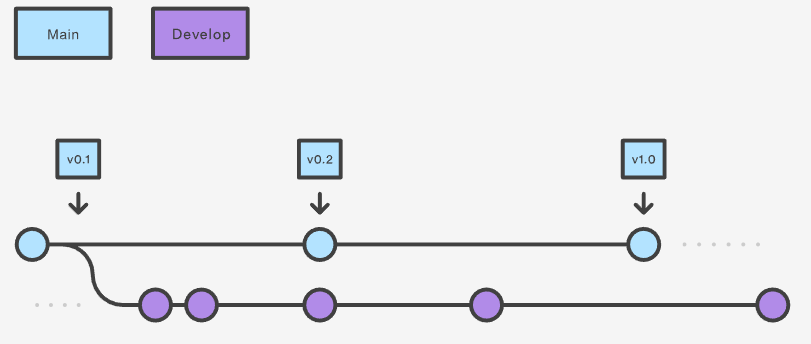
\includegraphics[width=0.7\textwidth]{gitflow1.png}
            \attribution{https://www.atlassian.com/git/tutorials/comparing-workflows/gitflow-workflow}
        \end{center}
        \begin{itemize}
            \item master --- история релизов
            \item develop --- история разработки
        \end{itemize}
    \end{frame}

    \begin{frame}
        \frametitle{Gitflow, feature-ветки}
        \begin{center}
            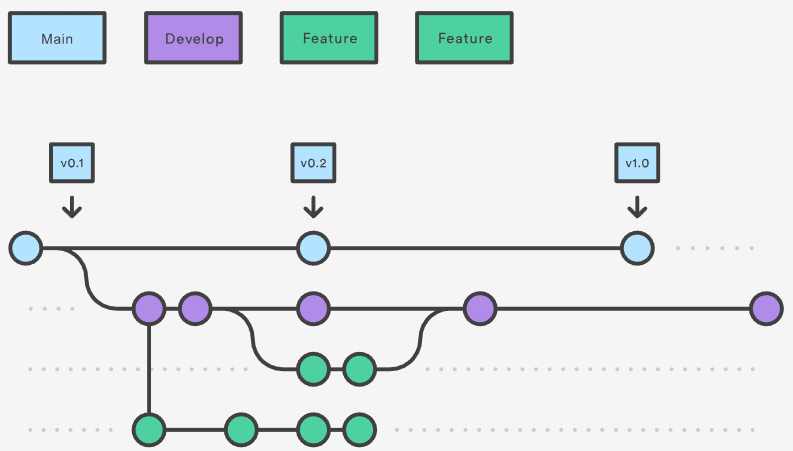
\includegraphics[width=0.7\textwidth]{gitflow2.png}
            \attribution{https://www.atlassian.com/git/tutorials/comparing-workflows/gitflow-workflow}
        \end{center}
        \begin{itemize}
            \item feature-ветки --- отводятся от develop
            \item Для разработки функциональности и правки багов
        \end{itemize}
    \end{frame}

    \begin{frame}
        \frametitle{Gitflow, релизные ветки}
        \begin{center}
            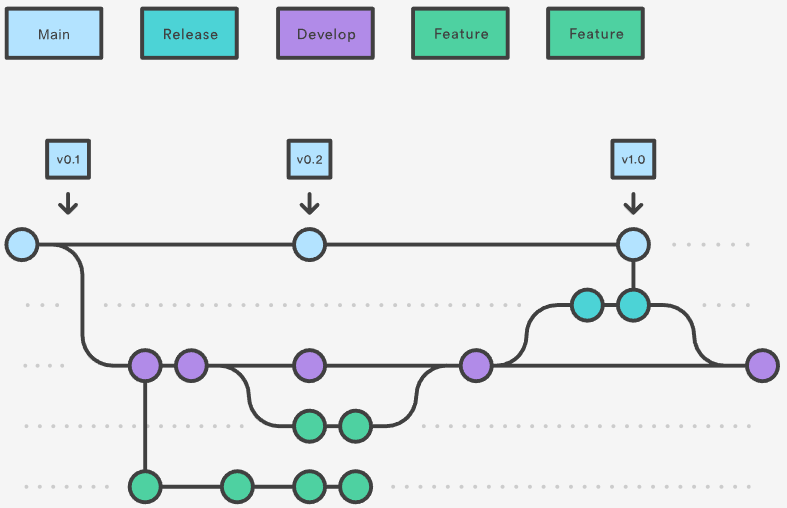
\includegraphics[width=0.7\textwidth]{gitflow3.png}
            \attribution{https://www.atlassian.com/git/tutorials/comparing-workflows/gitflow-workflow}
        \end{center}
        \begin{itemize}
            \item Релизные ветки --- для исправления багов перед релизом
            \item Чтобы ``заморозить'' код
        \end{itemize}
    \end{frame}

    \begin{frame}
        \frametitle{Gitflow, хотфиксы}
        \begin{center}
            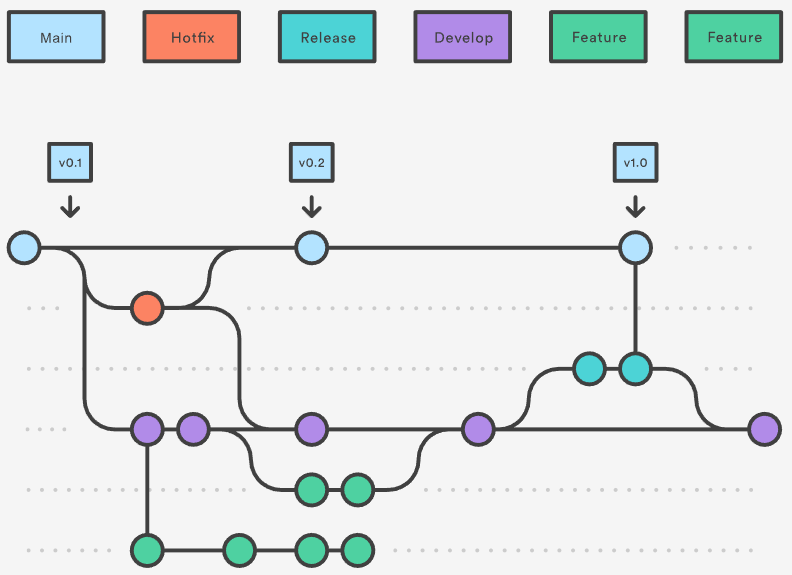
\includegraphics[width=0.6\textwidth]{gitflow4.png}
            \attribution{https://www.atlassian.com/git/tutorials/comparing-workflows/gitflow-workflow}
        \end{center}
        \begin{itemize}
            \item Хотфикс-ветки --- отводятся от main
            \item Для правки багов в уже выпущенном коде
        \end{itemize}
    \end{frame}

    \begin{frame}
        \frametitle{Gitflow}
        \begin{itemize}
            \item Хорошо подходит для поддержки больших проектов
            \item Сложное слияние изменений, не очень актуальный код в develop
            \item Трудночитаемая история
            \item Затрудняет CI/CD
        \end{itemize}
    \end{frame}

    \subsection{GitHub flow}

    \begin{frame}
        \frametitle{GitHub flow}
        \begin{center}
            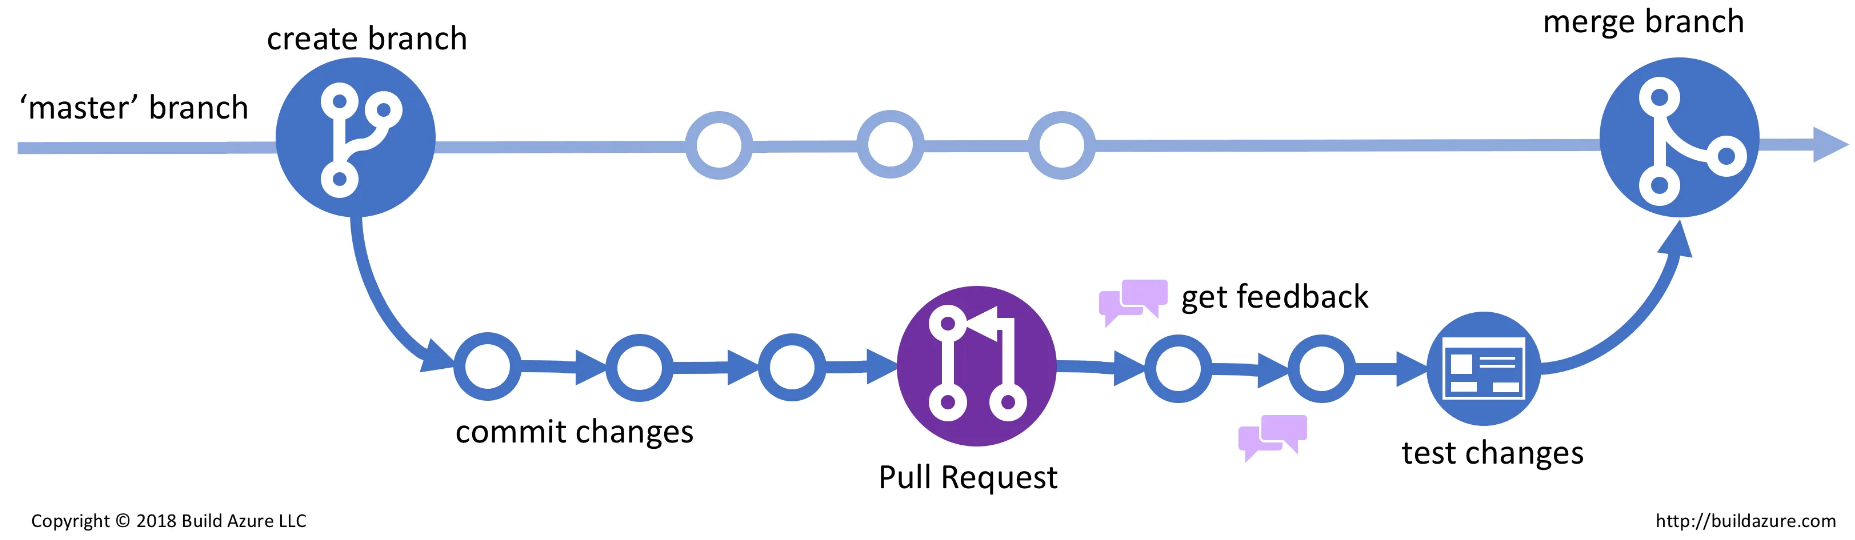
\includegraphics[width=0.95\textwidth]{gitHubFlow.png}
        \end{center}
        \begin{itemize}
            \item Без develop
            \item Пуллреквесты для слияния
            \item Вариант с fork-репозиториями
        \end{itemize}
    \end{frame}

    \begin{frame}
        \frametitle{Gitflow}
        \begin{itemize}
            \item Легко сломать главную ветку
            \item Проще
            \item Проще CI/CD
        \end{itemize}
    \end{frame}

    \subsection{Gitlab flow}

    \begin{frame}
        \frametitle{GitLab flow}
        \begin{columns}
            \begin{column}{0.6\textwidth}
                \begin{itemize}
                    \item Упор на развёртывание
                    \item Коммиты в главную ветку автоматически развёртываются в тестовом окружении
                    \item Развёртывание в production --- вручную
                \end{itemize}
            \end{column}
            \begin{column}{0.4\textwidth}
                \begin{center}
                    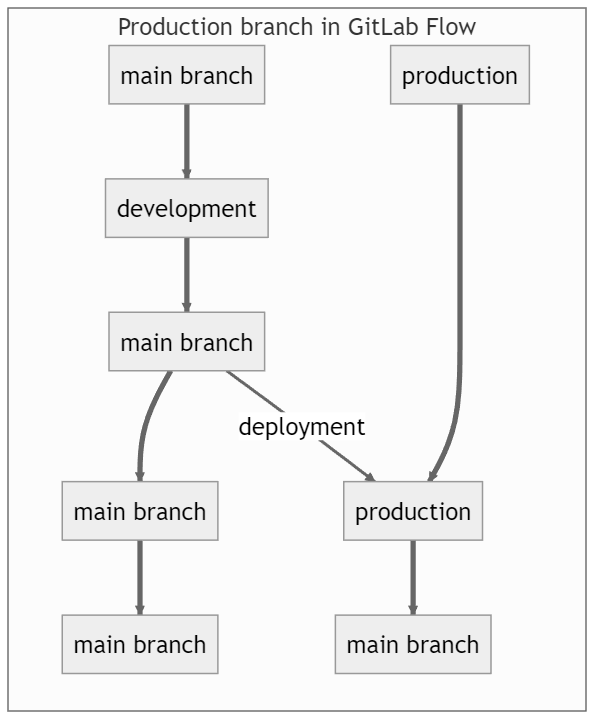
\includegraphics[height=0.6\textheight]{gitlabFlow.png}
                \end{center}
            \end{column}
        \end{columns}
        \attribution{https://docs.gitlab.com/ee/topics/gitlab\_flow.html}
    \end{frame}

    \begin{frame}
        \frametitle{GitLab flow, ветки окружения}
        \begin{center}
            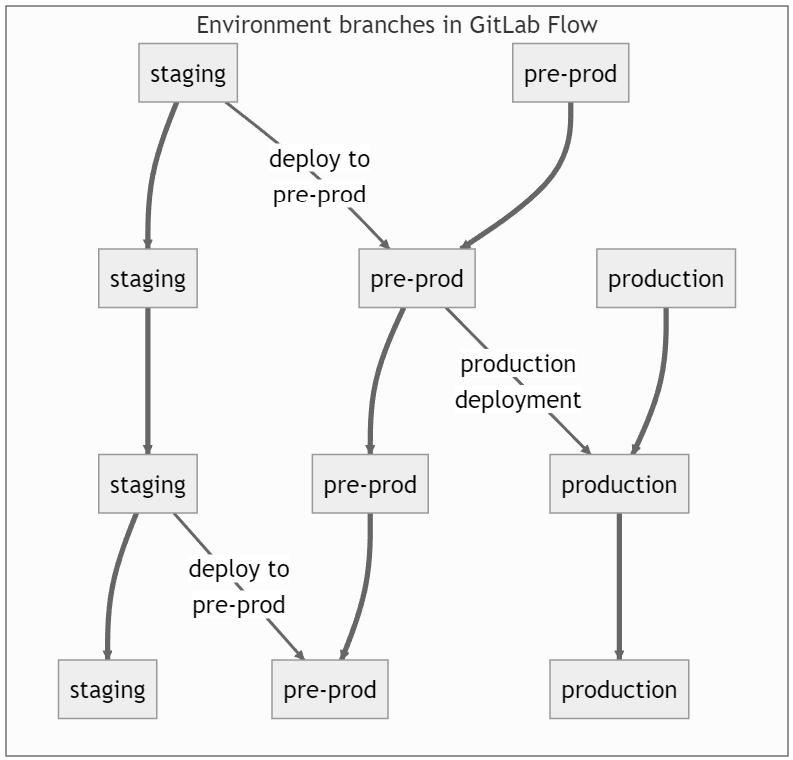
\includegraphics[width=0.45\textwidth]{gitlabFlow2.png}
            \attribution{https://docs.gitlab.com/ee/topics/gitlab\_flow.html}
        \end{center}
        \begin{itemize}
            \item Pre-prod и staging --- два окружения для тестирования и развёртывания
            \item Могут быть релизные ветки
        \end{itemize}
    \end{frame}

    \begin{frame}
        \frametitle{GitLab flow}
        \begin{itemize}
            \item Продвинутый CI/CD в нескольких окружениях
            \item Не так удобно поддерживать несколько веток
        \end{itemize}
    \end{frame}

    \subsection{OneFlow}

    \begin{frame}
        \frametitle{OneFlow}
        \begin{columns}
            \begin{column}{0.4\textwidth}
                \begin{itemize}
                    \item Главная ветка, feature-ветки
                    \item Три способа слияния
                    \item Первый --- rebase
                \end{itemize}
            \end{column}
            \begin{column}{0.6\textwidth}
                \begin{center}
                    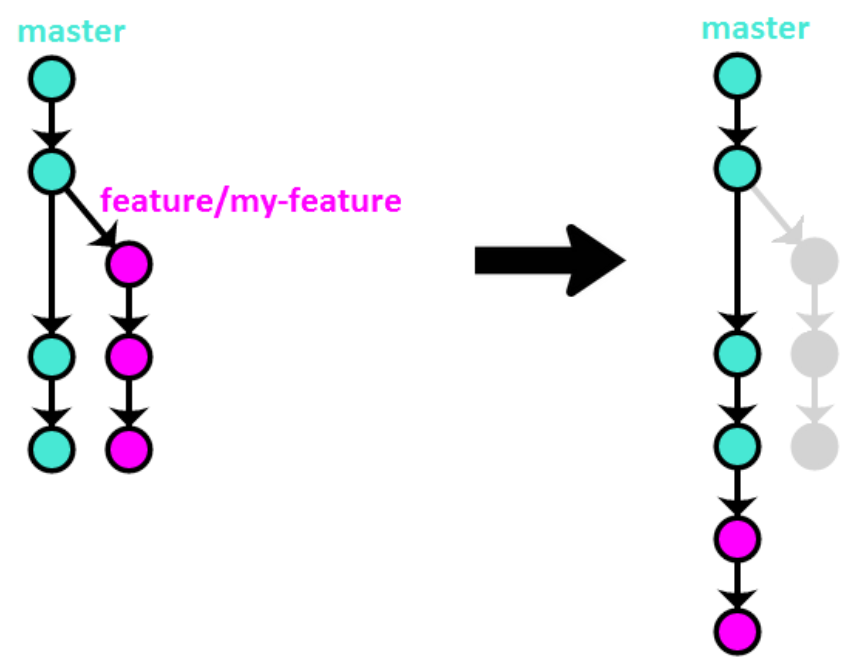
\includegraphics[width=0.9\textwidth]{oneflow1.png}
                    \attribution{https://www.endoflineblog.com/oneflow-a-git-branching-model-and-workflow}
                \end{center}
            \end{column}
        \end{columns}
    \end{frame}

    \begin{frame}
        \frametitle{OneFlow}
        \begin{columns}
            \begin{column}{0.4\textwidth}
                \begin{itemize}
                    \item Второй --- merge
                \end{itemize}
            \end{column}
            \begin{column}{0.6\textwidth}
                \begin{center}
                    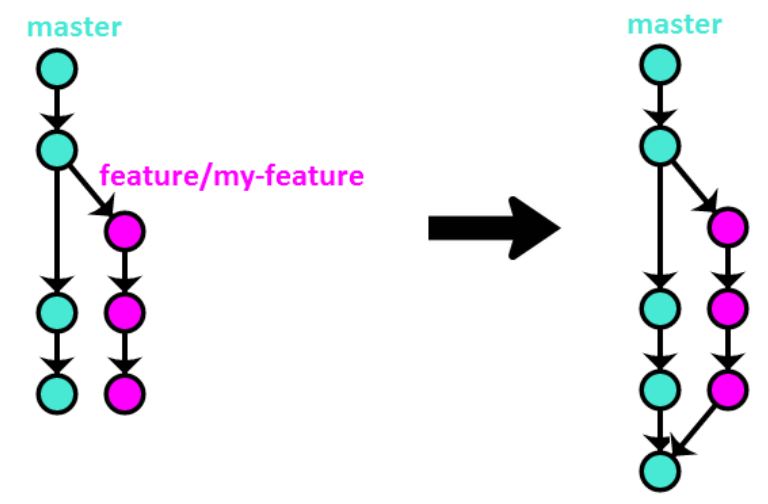
\includegraphics[width=0.9\textwidth]{oneflow2.png}
                    \attribution{https://www.endoflineblog.com/oneflow-a-git-branching-model-and-workflow}
                \end{center}
            \end{column}
        \end{columns}
    \end{frame}

    \begin{frame}
        \frametitle{OneFlow}
        \begin{columns}
            \begin{column}{0.4\textwidth}
                \begin{itemize}
                    \item Третий --- rebase и merge
                \end{itemize}
            \end{column}
            \begin{column}{0.6\textwidth}
                \begin{center}
                    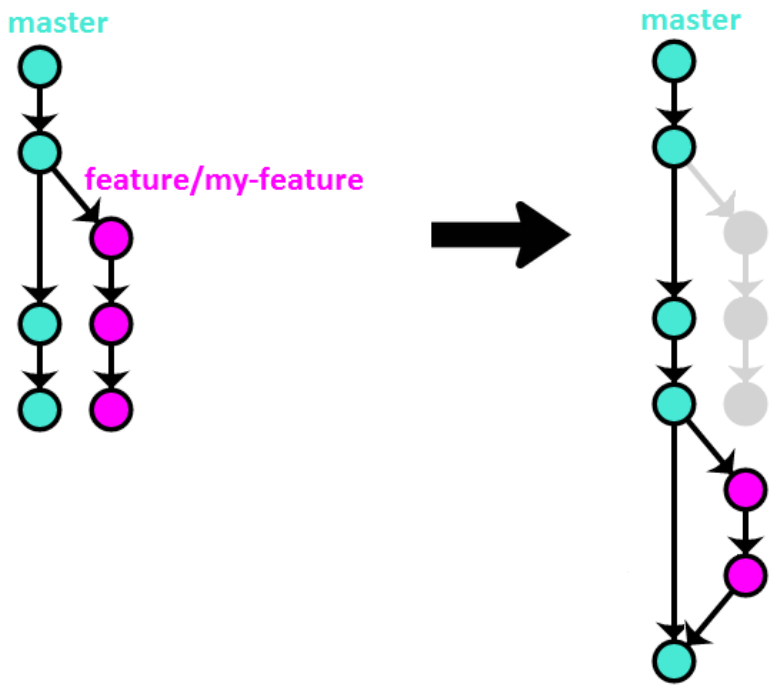
\includegraphics[width=0.9\textwidth]{oneflow3.png}
                    \attribution{https://www.endoflineblog.com/oneflow-a-git-branching-model-and-workflow}
                \end{center}
            \end{column}
        \end{columns}
    \end{frame}

    \begin{frame}
        \frametitle{OneFlow, релизные ветки}
        \begin{columns}
            \begin{column}{0.4\textwidth}
                \begin{itemize}
                    \item Релизные ветки --- от основной
                    \item После релиза --- тэг и слияние в основную
                \end{itemize}
            \end{column}
            \begin{column}{0.6\textwidth}
                \begin{center}
                    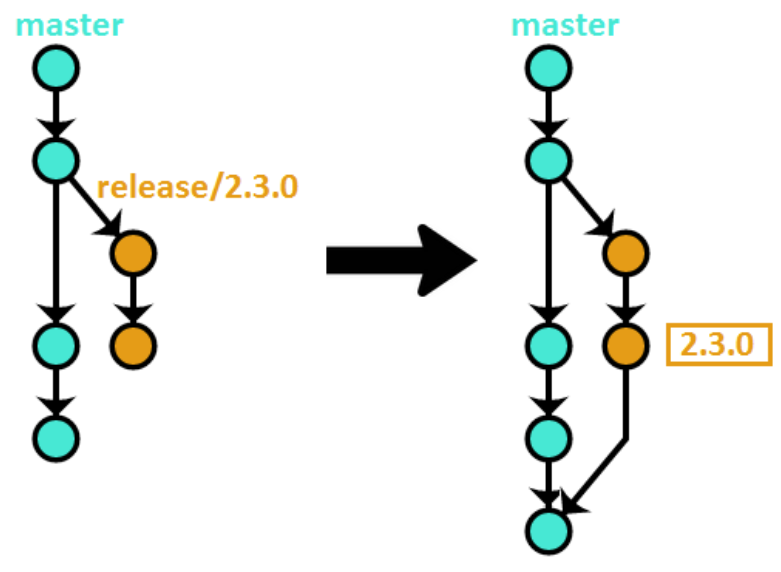
\includegraphics[width=0.9\textwidth]{oneflow4.png}
                    \attribution{https://www.endoflineblog.com/oneflow-a-git-branching-model-and-workflow}
                \end{center}
            \end{column}
        \end{columns}
    \end{frame}

    \begin{frame}
        \frametitle{OneFlow, хотфиксы}
        \begin{columns}
            \begin{column}{0.4\textwidth}
                \begin{itemize}
                    \item Хотфиксы --- от релизной ветки
                    \item После релиза --- тэг и слияние в основную
                \end{itemize}
            \end{column}
            \begin{column}{0.6\textwidth}
                \begin{center}
                    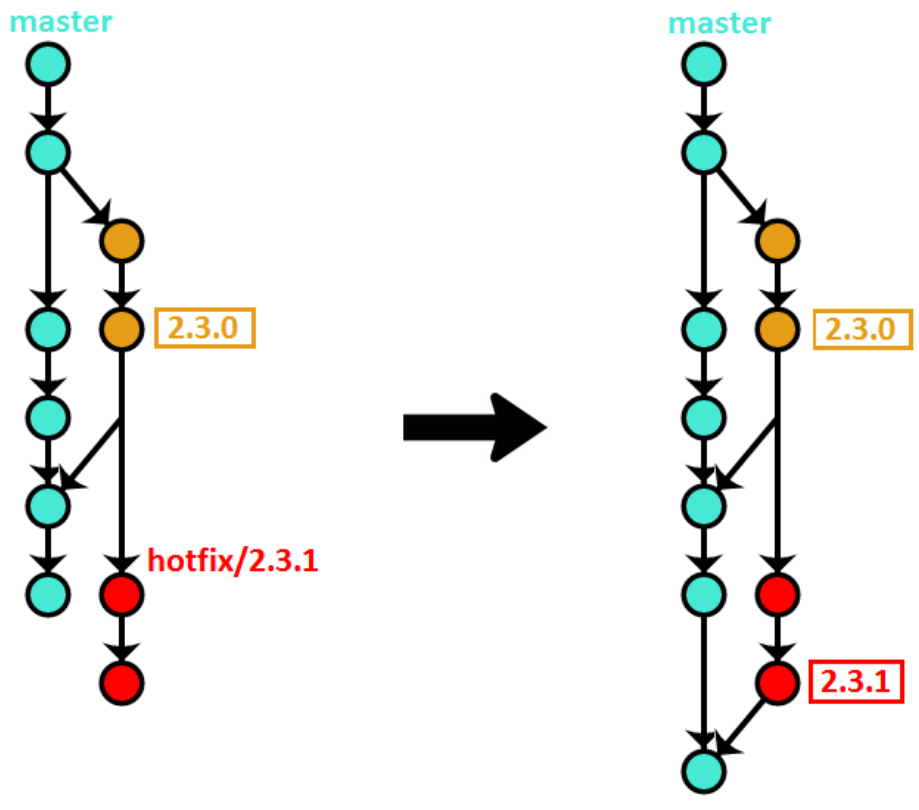
\includegraphics[height=0.7\textheight]{oneflow5.png}
                    \attribution{https://www.endoflineblog.com/oneflow-a-git-branching-model-and-workflow}
                \end{center}
            \end{column}
        \end{columns}
    \end{frame}

    \begin{frame}
        \frametitle{OneFlow}
        \begin{itemize}
            \item Прямолинейная история коммитов
            \item Нетривиальный CI/CD
            \item Сложно поддерживать несколько версий
        \end{itemize}
    \end{frame}

\end{document}
